\documentclass{article}\usepackage[]{graphicx}\usepackage[]{color}
% maxwidth is the original width if it is less than linewidth
% otherwise use linewidth (to make sure the graphics do not exceed the margin)
\makeatletter
\def\maxwidth{ %
  \ifdim\Gin@nat@width>\linewidth
    \linewidth
  \else
    \Gin@nat@width
  \fi
}
\makeatother

\definecolor{fgcolor}{rgb}{0.345, 0.345, 0.345}
\newcommand{\hlnum}[1]{\textcolor[rgb]{0.686,0.059,0.569}{#1}}%
\newcommand{\hlstr}[1]{\textcolor[rgb]{0.192,0.494,0.8}{#1}}%
\newcommand{\hlcom}[1]{\textcolor[rgb]{0.678,0.584,0.686}{\textit{#1}}}%
\newcommand{\hlopt}[1]{\textcolor[rgb]{0,0,0}{#1}}%
\newcommand{\hlstd}[1]{\textcolor[rgb]{0.345,0.345,0.345}{#1}}%
\newcommand{\hlkwa}[1]{\textcolor[rgb]{0.161,0.373,0.58}{\textbf{#1}}}%
\newcommand{\hlkwb}[1]{\textcolor[rgb]{0.69,0.353,0.396}{#1}}%
\newcommand{\hlkwc}[1]{\textcolor[rgb]{0.333,0.667,0.333}{#1}}%
\newcommand{\hlkwd}[1]{\textcolor[rgb]{0.737,0.353,0.396}{\textbf{#1}}}%
\let\hlipl\hlkwb

\usepackage{framed}
\makeatletter
\newenvironment{kframe}{%
 \def\at@end@of@kframe{}%
 \ifinner\ifhmode%
  \def\at@end@of@kframe{\end{minipage}}%
  \begin{minipage}{\columnwidth}%
 \fi\fi%
 \def\FrameCommand##1{\hskip\@totalleftmargin \hskip-\fboxsep
 \colorbox{shadecolor}{##1}\hskip-\fboxsep
     % There is no \\@totalrightmargin, so:
     \hskip-\linewidth \hskip-\@totalleftmargin \hskip\columnwidth}%
 \MakeFramed {\advance\hsize-\width
   \@totalleftmargin\z@ \linewidth\hsize
   \@setminipage}}%
 {\par\unskip\endMakeFramed%
 \at@end@of@kframe}
\makeatother

\definecolor{shadecolor}{rgb}{.97, .97, .97}
\definecolor{messagecolor}{rgb}{0, 0, 0}
\definecolor{warningcolor}{rgb}{1, 0, 1}
\definecolor{errorcolor}{rgb}{1, 0, 0}
\newenvironment{knitrout}{}{} % an empty environment to be redefined in TeX

\usepackage{alltt}
\usepackage[margin = 2cm]{geometry}
\usepackage{hyperref}
\usepackage[parfill]{parskip}
\usepackage{amsfonts, amsmath}
\usepackage{placeins}


\title{Lab 1: Correlation and Linear Regression}
\author{}
\IfFileExists{upquote.sty}{\usepackage{upquote}}{}
\begin{document}
\maketitle  

Today we will be reviewing various data sets having to do with the Buffalo Bills and US presidential elections. Our goals for this week are

\begin{itemize}
\item Review concepts about regression and correlation
\item Introduce the `lm` function
\item Examining the effect of outliers
\end{itemize}

\section{Best Fitting Line: Buffalo Bills}

The Buffalo Bills are a team in the National Football League based out of Buffalo, NY. To review a few points about regression, we'll consider the weight and height of the Buffalo Bills roster. First, let's read in the data and plot what it looks like.


\begin{knitrout}
\definecolor{shadecolor}{rgb}{0.969, 0.969, 0.969}\color{fgcolor}\begin{kframe}
\begin{alltt}
\hlcom{## package which allows you to pull files directly from github}
\hlkwd{install.packages}\hlstd{(}\hlstr{"readr"}\hlstd{)}
\end{alltt}


{\ttfamily\noindent\itshape\color{messagecolor}{\#\# Installing package into '/home/ysw7/R/x86\_64-pc-linux-gnu-library/4.1'\\\#\# (as 'lib' is unspecified)}}\begin{alltt}
\hlkwd{library}\hlstd{(}\hlstr{"readr"}\hlstd{)}

\hlstd{fileName} \hlkwb{<-} \hlstr{"https://raw.githubusercontent.com/ysamwang/btry6020_sp22/main/lab1/buffaloBills.csv"}

\hlcom{# This pulls the data set into R, and assigns it to the variable `buffaloBills`}
\hlstd{buffaloBills} \hlkwb{<-} \hlkwd{read.csv}\hlstd{(}\hlkwd{url}\hlstd{(fileName))}
\end{alltt}
\end{kframe}
\end{knitrout}

Let's take a look at what's in the data. We can use the \texttt{head} function to view the first few lines of our data. 


\begin{knitrout}
\definecolor{shadecolor}{rgb}{0.969, 0.969, 0.969}\color{fgcolor}\begin{kframe}
\begin{alltt}
\hlcom{# The buffaloBills variable stores a table which contains information about each player.}
\hlcom{#The 'head' command shows the first few lines of the table}
\hlkwd{head}\hlstd{(buffaloBills)}
\end{alltt}
\begin{verbatim}
##          Player Number Position Height Weight Experience          College
## 1 Mario Addison     97       DE     75    260         11             Troy
## 2    Josh Allen     17       QB     77    237          4          Wyoming
## 3 Boogie Basham     96       DE     75    274          0      Wake Forest
## 4    Tyler Bass      2        K     70    183          2 Georgia Southern
## 5    Ryan Bates     71        G     76    302          3       Penn State
## 6  Cole Beasley     11       WR     68    174         10              SMU
\end{verbatim}
\begin{alltt}
\hlcom{# dim gets the size of the table}
\hlkwd{dim}\hlstd{(buffaloBills)}
\end{alltt}
\begin{verbatim}
## [1] 82  7
\end{verbatim}
\end{kframe}
\end{knitrout}

Given a table with multiple columns, we can use the \texttt{\$} operator to pull out specific columns. For example \texttt{buffaloBills\$Height} will return the \texttt{Height} column from \texttt{buffaloBills}. Notice for the \texttt{hist} command, we include the following arguments to label the plot (\texttt{main} is the main title, \texttt{ylab} is the label for the y-axis and \texttt{xlab} is the label for the x-axis). We can first view a histogram of the ''Height'' column which tells us how many times a specific number occured in our data set.

\begin{knitrout}
\definecolor{shadecolor}{rgb}{0.969, 0.969, 0.969}\color{fgcolor}\begin{kframe}
\begin{alltt}
\hlcom{# To reference a specific row in the table, you can use }
\hlcom{# the dollar sign and then use the column name. Note that it is case sensitive}
\hlstd{buffaloBills}\hlopt{$}\hlstd{Height}
\end{alltt}
\begin{verbatim}
##  [1] 75 77 75 70 76 68 70 80 76 74 77 72 72 80 77 78 76 74 75 72 72 72 77 74 72
## [26] 71 70 71 72 73 76 76 69 74 73 68 72 78 69 72 78 73 75 72 78 71 67 72 70 77
## [51] 74 72 78 70 75 75 74 77 74 74 73 72 73 75 78 75 73 74 72 77 71 69 78 75 71
## [76] 75 76 76 74 72 77 70
\end{verbatim}
\begin{alltt}
\hlkwd{hist}\hlstd{(buffaloBills}\hlopt{$}\hlstd{Height,} \hlkwc{main} \hlstd{=} \hlstr{"Histogram of Bills Height"}\hlstd{,}
     \hlkwc{ylab} \hlstd{=} \hlstr{"Occurences"}\hlstd{,} \hlkwc{xlab} \hlstd{=} \hlstr{"Inches"}\hlstd{)}
\end{alltt}
\end{kframe}

{\centering 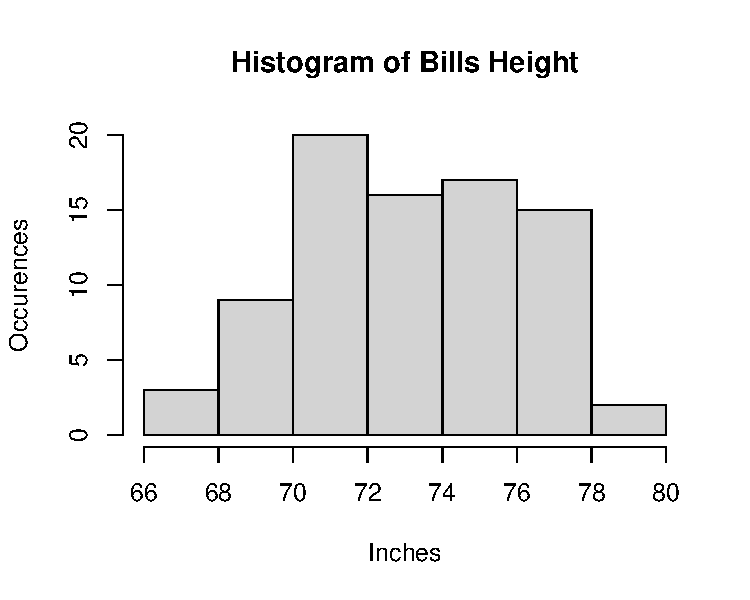
\includegraphics[width=\maxwidth]{figure/unnamed-chunk-3-1} 

}


\end{knitrout}

We can also grab specific elements of a vector using the the square brackets. 
\begin{knitrout}
\definecolor{shadecolor}{rgb}{0.969, 0.969, 0.969}\color{fgcolor}\begin{kframe}
\begin{alltt}
\hlcom{# To access the first element of the Height column}
\hlstd{buffaloBills}\hlopt{$}\hlstd{Height[}\hlnum{1}\hlstd{]}
\end{alltt}
\begin{verbatim}
## [1] 75
\end{verbatim}
\begin{alltt}
\hlcom{# To access the first 5 elements of the Height column}
\hlstd{buffaloBills}\hlopt{$}\hlstd{Height[}\hlkwd{c}\hlstd{(}\hlnum{1}\hlstd{,}\hlnum{2}\hlstd{,}\hlnum{3}\hlstd{,}\hlnum{4}\hlstd{,}\hlnum{5}\hlstd{)]}
\end{alltt}
\begin{verbatim}
## [1] 75 77 75 70 76
\end{verbatim}
\begin{alltt}
\hlstd{buffaloBills}\hlopt{$}\hlstd{Height[}\hlnum{1}\hlopt{:}\hlnum{5}\hlstd{]}
\end{alltt}
\begin{verbatim}
## [1] 75 77 75 70 76
\end{verbatim}
\begin{alltt}
\hlcom{# To access the all elements except for the first 5 elements of the Height column}
\hlstd{buffaloBills}\hlopt{$}\hlstd{Height[}\hlopt{-}\hlkwd{c}\hlstd{(}\hlnum{1}\hlstd{,}\hlnum{2}\hlstd{,}\hlnum{3}\hlstd{,}\hlnum{4}\hlstd{,}\hlnum{5}\hlstd{)]}
\end{alltt}
\begin{verbatim}
##  [1] 68 70 80 76 74 77 72 72 80 77 78 76 74 75 72 72 72 77 74 72 71 70 71 72 73
## [26] 76 76 69 74 73 68 72 78 69 72 78 73 75 72 78 71 67 72 70 77 74 72 78 70 75
## [51] 75 74 77 74 74 73 72 73 75 78 75 73 74 72 77 71 69 78 75 71 75 76 76 74 72
## [76] 77 70
\end{verbatim}
\begin{alltt}
\hlcom{# To access the 3rd row of the buffaloBills table}
\hlstd{buffaloBills[}\hlnum{3}\hlstd{, ]}
\end{alltt}
\begin{verbatim}
##          Player Number Position Height Weight Experience     College
## 3 Boogie Basham     96       DE     75    274          0 Wake Forest
\end{verbatim}
\begin{alltt}
\hlcom{# To access the 4th column of the buffaloBills table}
\hlstd{buffaloBills[,} \hlnum{4}\hlstd{]}
\end{alltt}
\begin{verbatim}
##  [1] 75 77 75 70 76 68 70 80 76 74 77 72 72 80 77 78 76 74 75 72 72 72 77 74 72
## [26] 71 70 71 72 73 76 76 69 74 73 68 72 78 69 72 78 73 75 72 78 71 67 72 70 77
## [51] 74 72 78 70 75 75 74 77 74 74 73 72 73 75 78 75 73 74 72 77 71 69 78 75 71
## [76] 75 76 76 74 72 77 70
\end{verbatim}
\end{kframe}
\end{knitrout}



Suppose I am interested in the line which best describes the relationship between height (x variable) and weight (y variable) for the current Buffalo Bills roster. Thus, my \textbf{population} of interest is the current Bills roster. Thus, in this case, I can actually calculate my \textbf{parameters} of interest, the $b_0$ and $b_1$ which minimize the sum of squared residuals, because I have access to the entire population (note this is typically not the case).

We can use the \texttt{cov}, \texttt{var}, and \texttt{mean} functions to calculate the relevant sample quantities.
\begin{knitrout}
\definecolor{shadecolor}{rgb}{0.969, 0.969, 0.969}\color{fgcolor}\begin{kframe}
\begin{alltt}
\hlcom{# Using the formulas from class}
\hlstd{b1} \hlkwb{<-} \hlkwd{cov}\hlstd{(buffaloBills}\hlopt{$}\hlstd{Weight, buffaloBills}\hlopt{$}\hlstd{Height)} \hlopt{/} \hlkwd{var}\hlstd{(buffaloBills}\hlopt{$}\hlstd{Height)}
\hlstd{b0} \hlkwb{<-} \hlkwd{mean}\hlstd{(buffaloBills}\hlopt{$}\hlstd{Weight)} \hlopt{-} \hlstd{b1} \hlopt{*} \hlkwd{mean}\hlstd{(buffaloBills}\hlopt{$}\hlstd{Height)}

\hlcom{# Population parameters}
\hlstd{b0}
\end{alltt}
\begin{verbatim}
## [1] -730.2878
\end{verbatim}
\begin{alltt}
\hlstd{b1}
\end{alltt}
\begin{verbatim}
## [1] 13.17275
\end{verbatim}
\end{kframe}
\end{knitrout}
So our estimated regression model would be
\begin{equation}
\text{Weight}_i = -730.2878 + 13.1725 \times \text{Height} + \epsilon_i
\end{equation}

\subsubsection*{Questions}
\begin{itemize}
\item How should we interpret these parameters?
\end{itemize}


\vspace{1em}

Using these values, we can create predictions for each player's weight based on their height. We can also calculate the residual and check that the sum of the residuals is 0 as we claimed in class. 
\begin{knitrout}
\definecolor{shadecolor}{rgb}{0.969, 0.969, 0.969}\color{fgcolor}\begin{kframe}
\begin{alltt}
\hlstd{y.hat} \hlkwb{<-} \hlstd{b0} \hlopt{+} \hlstd{b1} \hlopt{*} \hlstd{buffaloBills}\hlopt{$}\hlstd{Height}
\hlstd{residual} \hlkwb{<-} \hlstd{buffaloBills}\hlopt{$}\hlstd{Weight} \hlopt{-} \hlstd{y.hat}
\hlkwd{sum}\hlstd{(residual)}
\end{alltt}
\begin{verbatim}
## [1] 3.637979e-12
\end{verbatim}
\end{kframe}
\end{knitrout}


Now let's check to see that these values of $b_0$ and $b_1$ actually mimimize the sum of squared errors 
\begin{equation}
\text{RSS} = \sum_i (y_i - \hat y_i)^2
\end{equation}
To do this, let's first calculate the RSS for our current estimates of $b_0$ and $b_1$
\begin{knitrout}
\definecolor{shadecolor}{rgb}{0.969, 0.969, 0.969}\color{fgcolor}\begin{kframe}
\begin{alltt}
\hlkwd{sum}\hlstd{(residual}\hlopt{^}\hlnum{2}\hlstd{)}
\end{alltt}
\begin{verbatim}
## [1] 83857.67
\end{verbatim}
\end{kframe}
\end{knitrout}

Now let's take a quick eyeball at the plot, and select a value for $b_0$ and $b_1$ (pretend you don't know the actual values we just calculated). I've filled in a guess, but you should change the code to your own values for \texttt{b0.guess} and \texttt{b1.guess}

\begin{knitrout}
\definecolor{shadecolor}{rgb}{0.969, 0.969, 0.969}\color{fgcolor}\begin{kframe}
\begin{alltt}
\hlstd{b0.guess} \hlkwb{<-} \hlopt{-}\hlnum{110}
\hlstd{b1.guess} \hlkwb{<-} \hlnum{5}
\hlstd{y.hat.guess} \hlkwb{<-} \hlstd{b0.guess} \hlopt{+} \hlstd{b1.guess} \hlopt{*} \hlstd{buffaloBills}\hlopt{$}\hlstd{Height}
\hlstd{residual.guess} \hlkwb{<-} \hlstd{buffaloBills}\hlopt{$}\hlstd{Weight} \hlopt{-} \hlstd{y.hat.guess}
\hlkwd{sum}\hlstd{(residual.guess}\hlopt{^}\hlnum{2}\hlstd{)}
\end{alltt}
\begin{verbatim}
## [1] 155447
\end{verbatim}
\end{kframe}
\end{knitrout}

\subsubsection*{Questions}
\begin{itemize}
\item What is the RSS for your ``guessed" values of $b_0$ and $b_1$?
\item Is it less than the  for the least squares values of $b_0$ and $b_1$?
\end{itemize}

However, let's suppose I didn't have data for the full roster, but instead I needed to gather it myself. I ask Sean McDermott, the Bills Coach, and he says I can get the data from the players. However, since they're in the middle of the season and he doesn't want to distract the players, he says I can only ask 10 of the players, not the entire team. So I randomly select 10 players out of the 82 listed on the roster and get the following data. 

To simulate this hypothetical situation happen, we first use the \texttt{sample} function which picks 10 random numbers between 1 and 82 (the number of players on the roster). Note that \texttt{c(1:82)} is shorthand for a vector containing all whole numbers between 1 and 82. 
\begin{knitrout}
\definecolor{shadecolor}{rgb}{0.969, 0.969, 0.969}\color{fgcolor}\begin{kframe}
\begin{alltt}
\hlstd{players} \hlkwb{<-} \hlkwd{sample}\hlstd{(}\hlkwd{c}\hlstd{(}\hlnum{1}\hlopt{:}\hlnum{82}\hlstd{),} \hlkwc{size} \hlstd{=} \hlnum{10}\hlstd{)}

\hlcom{# Set of players we selected. This is will be our sample}
\hlstd{players}
\end{alltt}
\begin{verbatim}
##  [1] 76 36 57 64 56 59 42 29 54 48
\end{verbatim}
\begin{alltt}
\hlstd{buffaloBills[players, ]}
\end{alltt}
\begin{verbatim}
##             Player Number Position Height Weight Experience            College
## 76   Justin Zimmer     61       DT     75    300          3       Ferris State
## 36 Isaiah McKenzie     19       WR     68    173          5            Georgia
## 57  Brandin Bryant     90       DT     74    305          1   Florida Atlantic
## 64  Isaiah Hodgins     16       WR     75    201          2       Oregon State
## 56       Eli Ankou     51       NT     75    325          5               UCLA
## 59   Tanner Gentry     87       WR     74    209          1            Wyoming
## 42       Ed Oliver     91       DT     73    287          3            Houston
## 29    Taiwan Jones     25       RB     72    195         11 Eastern Washington
## 54   Austin Proehl     NA       WR     70    175          1     North Carolina
## 48     Andre Smith     59       LB     72    240          4     North Carolina
\end{verbatim}
\end{kframe}
\end{knitrout}

We then fit a regression to the data from the 10 players selected. The 10 players that we would select is our \textbf{sample}, and the $\hat a$ and $\hat b$ we would get from only measuring 10 players are \textbf{statistics} which describe our sample.
\begin{knitrout}
\definecolor{shadecolor}{rgb}{0.969, 0.969, 0.969}\color{fgcolor}\begin{kframe}
\begin{alltt}
\hlstd{b1.hat} \hlkwb{<-} \hlkwd{cov}\hlstd{(buffaloBills}\hlopt{$}\hlstd{Weight[players], buffaloBills}\hlopt{$}\hlstd{Height[players])} \hlopt{/}
  \hlkwd{var}\hlstd{(buffaloBills}\hlopt{$}\hlstd{Height[players])}
\hlstd{b0.hat} \hlkwb{<-} \hlkwd{mean}\hlstd{(buffaloBills}\hlopt{$}\hlstd{Weight[players])} \hlopt{-} \hlstd{b1.hat} \hlopt{*} \hlkwd{mean}\hlstd{(buffaloBills}\hlopt{$}\hlstd{Height[players])}

\hlcom{# The statistics we calculate from our sample}
\hlstd{b1.hat}
\end{alltt}
\begin{verbatim}
## [1] 16.59274
\end{verbatim}
\begin{alltt}
\hlstd{b0.hat}
\end{alltt}
\begin{verbatim}
## [1] -966.9516
\end{verbatim}
\end{kframe}
\end{knitrout}

\subsubsection*{Questions}
\begin{itemize}
\item Try this out yourself by running the code. You will get a different answer because your sample will probably be different from mine.
\item How do these values differ from our parameters calculated above?
\item Should I use the 'population values' from the Buffalo Bills roster to make predictions about the average American adult? Would you expect the `population values' for the American adult population be different?
\end{itemize}

Let's see how these values differ as we take many random samples. To do this, we will use a for loop which repeats a block of code. Each time it repeats the block, it sets  an index variable (in this case $i$) to the next value in the specified vector. We will repeat this procedure 500 times. We also create two vectors (record.b0 and record.b1) to record the estimates values of $\hat b_0$ and $\hat b_1$ for each sample  

\begin{knitrout}
\definecolor{shadecolor}{rgb}{0.969, 0.969, 0.969}\color{fgcolor}\begin{kframe}
\begin{alltt}
\hlstd{sample.size} \hlkwb{<-} \hlnum{500}
\hlstd{record.b0} \hlkwb{<-} \hlkwd{rep}\hlstd{(}\hlnum{0}\hlstd{, sample.size)}
\hlstd{record.b1} \hlkwb{<-} \hlkwd{rep}\hlstd{(}\hlnum{0}\hlstd{, sample.size)}

\hlcom{### Test out to see how a for loop works}
\hlcom{# for(i in 1:5)\{}
\hlcom{#  print(i^2)}
\hlcom{# \}}

\hlkwa{for}\hlstd{(i} \hlkwa{in} \hlkwd{c}\hlstd{(}\hlnum{1}\hlopt{:}\hlstd{sample.size))\{}

  \hlcom{# Set of players we selected. This is will be our sample}
  \hlstd{players} \hlkwb{<-} \hlkwd{sample}\hlstd{(}\hlkwd{c}\hlstd{(}\hlnum{1}\hlopt{:}\hlkwd{dim}\hlstd{(buffaloBills)[}\hlnum{1}\hlstd{]),} \hlkwc{size} \hlstd{=} \hlnum{10}\hlstd{)}

  \hlcom{# calculate the statistics}
  \hlstd{b1.hat} \hlkwb{<-} \hlkwd{cov}\hlstd{(buffaloBills}\hlopt{$}\hlstd{Weight[players], buffaloBills}\hlopt{$}\hlstd{Height[players])} \hlopt{/}
    \hlkwd{var}\hlstd{(buffaloBills}\hlopt{$}\hlstd{Height[players])}

  \hlstd{b0.hat} \hlkwb{<-} \hlkwd{mean}\hlstd{(buffaloBills}\hlopt{$}\hlstd{Weight[players])} \hlopt{-} \hlstd{b1.hat} \hlopt{*} \hlkwd{mean}\hlstd{(buffaloBills}\hlopt{$}\hlstd{Height[players])}

  \hlcom{# record the statistics we calculate from our sample}
  \hlstd{record.b1[i]} \hlkwb{<-} \hlstd{b1.hat}
  \hlstd{record.b0[i]} \hlkwb{<-} \hlstd{b0.hat}
\hlstd{\}}
\end{alltt}
\end{kframe}
\end{knitrout}

We can plot the distribution of the estimated $\hat b_1$ and $\hat b_0$ values and see that they vary with each sample around the true value of $b_1$ and $b_0$ we calculated above. The parameter values are indicated with the red vertical lines in the plots below.

\begin{knitrout}
\definecolor{shadecolor}{rgb}{0.969, 0.969, 0.969}\color{fgcolor}\begin{kframe}
\begin{alltt}
\hlcom{# this arranges the plots together so there is 1 row and 2 columns}
\hlkwd{par}\hlstd{(}\hlkwc{mfrow} \hlstd{=} \hlkwd{c}\hlstd{(}\hlnum{1}\hlstd{,}\hlnum{2}\hlstd{))}

\hlkwd{hist}\hlstd{(record.b0,} \hlkwc{main} \hlstd{=} \hlstr{"Estimated b0"}\hlstd{)}
\hlkwd{abline}\hlstd{(}\hlkwc{v} \hlstd{= b0,} \hlkwc{col} \hlstd{=} \hlstr{"red"}\hlstd{)}
\hlkwd{hist}\hlstd{(record.b1,} \hlkwc{main} \hlstd{=} \hlstr{"Estimated b1"}\hlstd{)}
\hlkwd{abline}\hlstd{(}\hlkwc{v} \hlstd{= b1,} \hlkwc{col} \hlstd{=} \hlstr{"red"}\hlstd{)}
\end{alltt}
\end{kframe}

{\centering 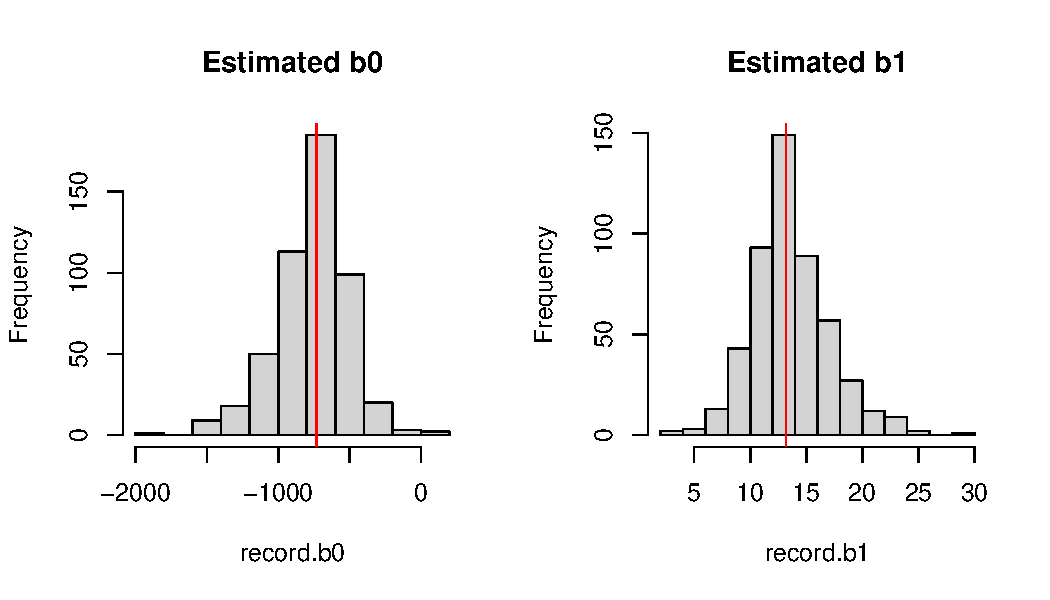
\includegraphics[width=\maxwidth]{figure/unnamed-chunk-12-1} 

}


\end{knitrout}

We can see that each random sample we take gives us a good estimate of the true values of $b_0$ and $b_1$, but $\hat b_0$ and $\hat b_1$ are different each time.


\newpage
\FloatBarrier


\section{Linear Models with US Presidential Elections}
In the 2000 US Presidential election with George Bush vs Al Gore, the entire election was decided by the state of Florida which itself was decided by less than 600 votes (a margin of .009\%). In particular, Palm Beach county used a butterfly ballot which was widely criticized for its confusing design. Many speculated that this may have caused a large number of voters who intended to vote for Al Gore to vote for Pat Buchanan (Reform Party) instead. 
 
\begin{figure}[h]
\centering
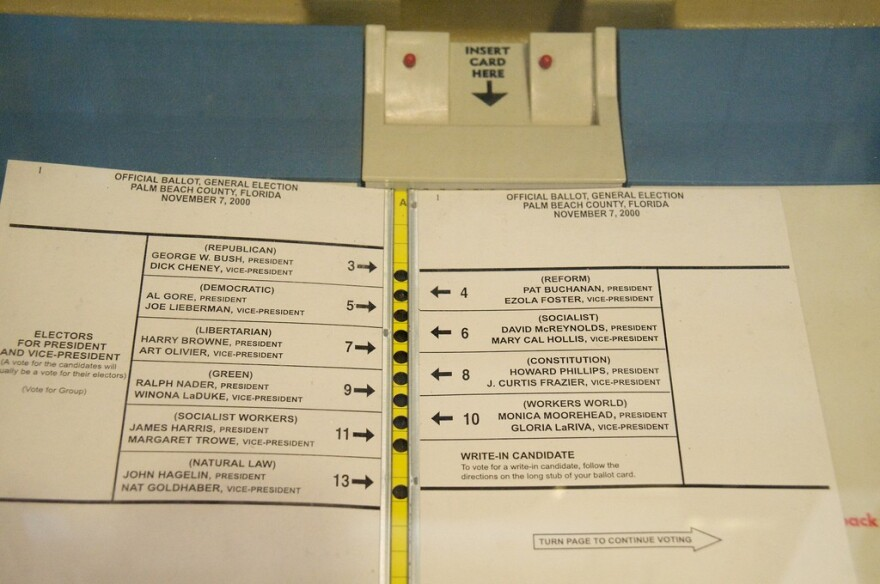
\includegraphics[scale = .3]{butterfly}
\caption{Confusing butterfly ballot}
\end{figure}

\FloatBarrier

We would expect that the number of registered voters in 2000 who belonged to the Reform party should be a pretty good predictor of how many people ended up voting for Pat Buchanan. For each county in Florida, we have combined vote data from Wikipedia with data from the Florida Division of Elections on the party affiliation of the registered voters in 2000. The variable \texttt{Buch.Votes} is the number of votes cast for Pat Buchannan and \texttt{Reg.Reform} is the number of registered reform party voters. \texttt{Total.Reg} is the total number of registered voters in that county. 

\begin{knitrout}
\definecolor{shadecolor}{rgb}{0.969, 0.969, 0.969}\color{fgcolor}\begin{kframe}
\begin{alltt}
\hlstd{fileName} \hlkwb{<-} \hlstr{"https://raw.githubusercontent.com/ysamwang/btry6020_sp22/main/lab1/FL.csv"}

\hlcom{# This pulls the data set into R, and assigns it to the variable `buffaloBills`}
\hlstd{florida} \hlkwb{<-} \hlkwd{read.csv}\hlstd{(}\hlkwd{url}\hlstd{(fileName))}

\hlkwd{head}\hlstd{(florida)}
\end{alltt}
\begin{verbatim}
##     County Reg.Dem Reg.Rep Reg.Reform Total.Reg Buch.Votes
## 1 Alachua    64135   34319         91    120867        263
## 2    Baker   10261    1684          4     12352         73
## 3      Bay   44209   34286         55     92749        268
## 4 Bradford    9639    2832          3     13547         45
## 5  Brevard  107840  131427        148    283680        570
## 6  Broward  456789  266829        332    887764        795
\end{verbatim}
\end{kframe}
\end{knitrout}

First, let's take a look at the distributions of registered reform party voters and votes for the reform party candidate Pat Buchannan. The red line in the plots below indicate the values for Palm County.

\begin{knitrout}
\definecolor{shadecolor}{rgb}{0.969, 0.969, 0.969}\color{fgcolor}\begin{kframe}
\begin{alltt}
\hlkwd{par}\hlstd{(}\hlkwc{mfrow} \hlstd{=} \hlkwd{c}\hlstd{(}\hlnum{1}\hlstd{,}\hlnum{3}\hlstd{))}

\hlcom{# Histogram of number of votes for Pat Buchannan}
\hlkwd{hist}\hlstd{(florida}\hlopt{$}\hlstd{Buch.Votes,} \hlkwc{main} \hlstd{=}  \hlstr{"Voters for Pat Buchannan by County"}\hlstd{)}
\hlkwd{abline}\hlstd{(}\hlkwc{v} \hlstd{= florida}\hlopt{$}\hlstd{Buch.Votes[}\hlnum{50}\hlstd{],} \hlkwc{col} \hlstd{=} \hlstr{"red"}\hlstd{)}

\hlcom{# Histogram of total registered reform party voters}
\hlkwd{hist}\hlstd{(florida}\hlopt{$}\hlstd{Reg.Reform,} \hlkwc{main} \hlstd{=} \hlstr{"Registered Reform Party Voters"}\hlstd{)}
\hlkwd{abline}\hlstd{(}\hlkwc{v} \hlstd{= florida}\hlopt{$}\hlstd{Reg.Reform[}\hlnum{50}\hlstd{],} \hlkwc{col} \hlstd{=} \hlstr{"red"}\hlstd{)}

\hlcom{# Normalize for the number of total registered voters}
\hlkwd{hist}\hlstd{(florida}\hlopt{$}\hlstd{Reg.Reform}\hlopt{/}\hlstd{florida}\hlopt{$}\hlstd{Total.Reg,}
     \hlkwc{main} \hlstd{=} \hlstr{"Registered Reform Party Voters"}\hlstd{)}
\hlkwd{abline}\hlstd{(}\hlkwc{v} \hlstd{= florida}\hlopt{$}\hlstd{Reg.Reform[}\hlnum{50}\hlstd{]}\hlopt{/}\hlstd{florida}\hlopt{$}\hlstd{Total.Reg[}\hlnum{50}\hlstd{],} \hlkwc{col} \hlstd{=} \hlstr{"red"}\hlstd{)}
\end{alltt}
\end{kframe}

{\centering 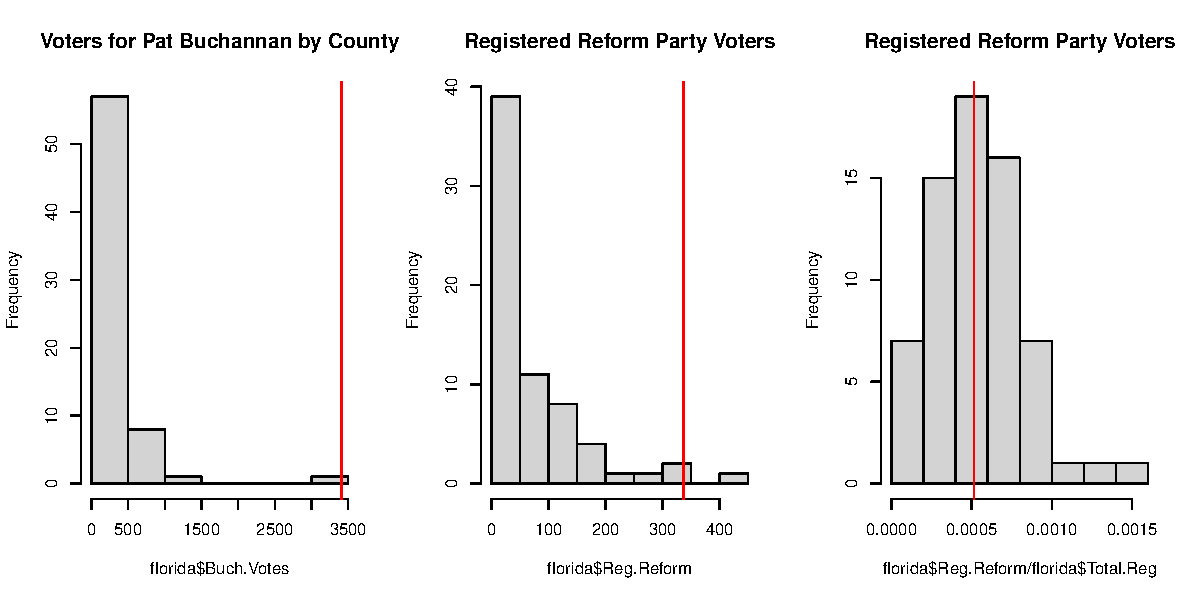
\includegraphics[width=\maxwidth]{figure/unnamed-chunk-14-1} 

}


\end{knitrout}

We can also plot the scatter plot, and use the \texttt{cor} function to calculate the sample correlation
\begin{knitrout}
\definecolor{shadecolor}{rgb}{0.969, 0.969, 0.969}\color{fgcolor}\begin{kframe}
\begin{alltt}
\hlkwd{plot}\hlstd{(florida}\hlopt{$}\hlstd{Reg.Reform, florida}\hlopt{$}\hlstd{Buch.Votes,}
     \hlkwc{xlab} \hlstd{=} \hlstr{"Registered Reform Party"}\hlstd{,} \hlkwc{ylab} \hlstd{=} \hlstr{"Votes for Buchannon"}\hlstd{,}
     \hlkwc{main} \hlstd{=} \hlstr{"Florida 2000 Presidential Election"}\hlstd{)}
\end{alltt}
\end{kframe}
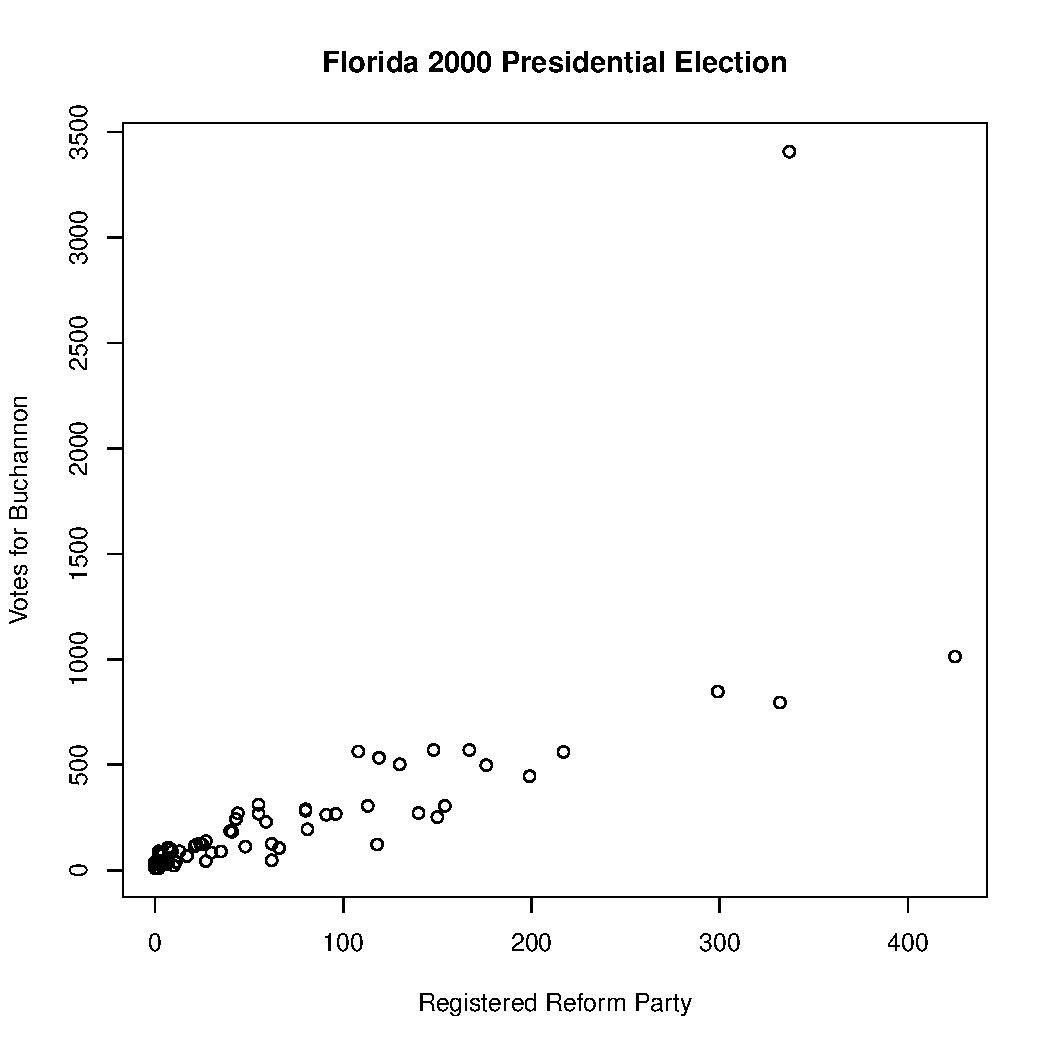
\includegraphics[width=\maxwidth]{figure/unnamed-chunk-15-1} 
\begin{kframe}\begin{alltt}
\hlkwd{round}\hlstd{(}\hlkwd{cor}\hlstd{(florida}\hlopt{$}\hlstd{Reg.Reform, florida}\hlopt{$}\hlstd{Buch.Votes),} \hlnum{3}\hlstd{)}
\end{alltt}
\begin{verbatim}
## [1] 0.741
\end{verbatim}
\end{kframe}
\end{knitrout}

\section{The \texttt{lm} function}

In the previous example, we formed the estimates of $\hat b_0$ and $\hat b_1$ by hand. We can also use the \texttt{lm} function (lm stands for linear model) to do all the work for us. Let's take the output of lm and assign it to the variable \texttt{reression.model}. Inside the \texttt{lm} function, we've specified the formula we want the function to fit. The response variable (y) is on the left side of the $\sim$ (it should be located next to the number 1 on your keyboard). On the right hand side of the tilde, we put the explanatory variable. We also specify the data frame which contains the data of interest.

Below, we calculate coefficients for the following model:
\begin{equation}
\text{votes for Buchannon}_i = b_0 + b_1 \text{number of registered reform party voters}_i + \epsilon_i
\end{equation}

\begin{knitrout}
\definecolor{shadecolor}{rgb}{0.969, 0.969, 0.969}\color{fgcolor}\begin{kframe}
\begin{alltt}
\hlstd{florida.regression} \hlkwb{=} \hlkwd{lm}\hlstd{(Buch.Votes} \hlopt{~} \hlstd{Reg.Reform,} \hlkwc{data} \hlstd{= florida)}
\end{alltt}
\end{kframe}
\end{knitrout}


We can get the fitted coefficients ($\hat b_0$ and $\hat b_1$) from the \texttt{florida.regression} object by using \texttt{\$coeff}. The first value is the y-intercept, and the second value is the coefficient on our explanatory variable (year.2004), which is denotes by $\hat b$ in the equation above. We can see that the values returned by \texttt{lm} are the same as the values we calculated above

\begin{knitrout}
\definecolor{shadecolor}{rgb}{0.969, 0.969, 0.969}\color{fgcolor}\begin{kframe}
\begin{alltt}
\hlstd{florida.regression}\hlopt{$}\hlstd{coeff}
\end{alltt}
\begin{verbatim}
## (Intercept)  Reg.Reform 
##   -0.246390    3.652078
\end{verbatim}
\begin{alltt}
\hlstd{b0.hat} \hlkwb{<-} \hlstd{florida.regression}\hlopt{$}\hlstd{coeff[}\hlnum{1}\hlstd{]}
\hlstd{b1.hat} \hlkwb{<-} \hlstd{florida.regression}\hlopt{$}\hlstd{coeff[}\hlnum{2}\hlstd{]}
\end{alltt}
\end{kframe}
\end{knitrout}

We can calculate predicted values using the estimated coefficients. Alternatively, we can get the predicted (or fitted values) from the \texttt{lm} object `florida.regression'.
\begin{knitrout}
\definecolor{shadecolor}{rgb}{0.969, 0.969, 0.969}\color{fgcolor}\begin{kframe}
\begin{alltt}
\hlstd{y.hat} \hlkwb{<-} \hlstd{b0.hat} \hlopt{+} \hlstd{b1.hat} \hlopt{*} \hlstd{florida}\hlopt{$}\hlstd{Reg.Reform}

\hlcom{# check to see that the predicted values we formed are the same as the}
\hlcom{# lm object's fitted values (at least up to 10 digits)}
\hlkwd{round}\hlstd{(florida.regression}\hlopt{$}\hlstd{fitted.values} \hlopt{-} \hlstd{y.hat,} \hlnum{10}\hlstd{)}
\end{alltt}
\begin{verbatim}
##  1  2  3  4  5  6  7  8  9 10 11 12 13 14 15 16 17 18 19 20 21 22 23 24 25 26 
##  0  0  0  0  0  0  0  0  0  0  0  0  0  0  0  0  0  0  0  0  0  0  0  0  0  0 
## 27 28 29 30 31 32 33 34 35 36 37 38 39 40 41 42 43 44 45 46 47 48 49 50 51 52 
##  0  0  0  0  0  0  0  0  0  0  0  0  0  0  0  0  0  0  0  0  0  0  0  0  0  0 
## 53 54 55 56 57 58 59 60 61 62 63 64 65 66 67 
##  0  0  0  0  0  0  0  0  0  0  0  0  0  0  0
\end{verbatim}
\end{kframe}
\end{knitrout}

In fact, the \texttt{lm} object has lots of information stored which we can access. To see, use the \texttt{names} function:
\begin{knitrout}
\definecolor{shadecolor}{rgb}{0.969, 0.969, 0.969}\color{fgcolor}\begin{kframe}
\begin{alltt}
\hlkwd{names}\hlstd{(florida.regression)}
\end{alltt}
\begin{verbatim}
##  [1] "coefficients"  "residuals"     "effects"       "rank"         
##  [5] "fitted.values" "assign"        "qr"            "df.residual"  
##  [9] "xlevels"       "call"          "terms"         "model"
\end{verbatim}
\end{kframe}
\end{knitrout}

Let's take a look at the observed values and the predicted values. To plot the line, we use the \texttt{abline} command which plots a line given the y-intercept (specified by the argument \texttt{a}) and the slope (specified by the argument \texttt{b}). It looks like the model fits relatively well.

\begin{knitrout}
\definecolor{shadecolor}{rgb}{0.969, 0.969, 0.969}\color{fgcolor}\begin{kframe}
\begin{alltt}
\hlkwd{plot}\hlstd{(florida}\hlopt{$}\hlstd{Reg.Reform, florida}\hlopt{$}\hlstd{Buch.Votes,} \hlkwc{main} \hlstd{=}\hlstr{"2000 Presidential Election Florida"}\hlstd{,}
     \hlkwc{xlab} \hlstd{=} \hlstr{"Registered Reform Party Voters"}\hlstd{,} \hlkwc{ylab} \hlstd{=} \hlstr{"Actual Reform Party Votes"}\hlstd{)}
\hlkwd{abline}\hlstd{(}\hlkwc{a} \hlstd{= b0.hat,} \hlkwc{b} \hlstd{= b1.hat,}
       \hlkwc{col} \hlstd{=} \hlstr{"red"}\hlstd{,} \hlkwc{lwd} \hlstd{=} \hlnum{2}\hlstd{)}
\end{alltt}
\end{kframe}

{\centering 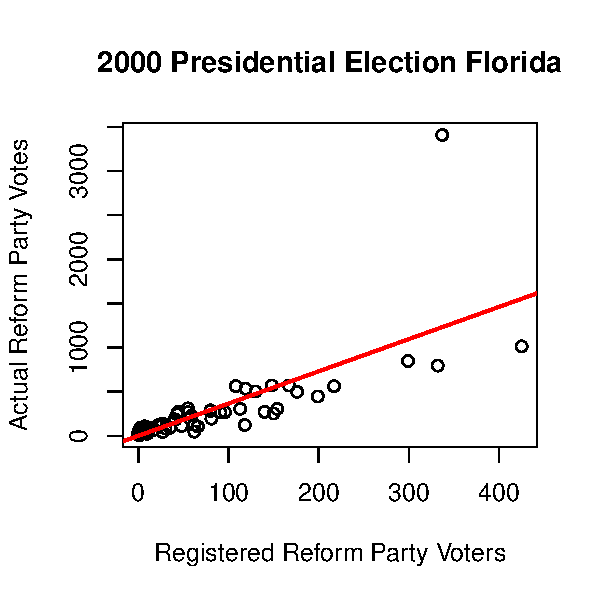
\includegraphics[width=\maxwidth]{figure/unnamed-chunk-20-1} 

}


\end{knitrout}

\subsubsection*{Questions}
\begin{itemize}
\item Does the line fit well? Does the relationship look mostly linear? 
\item Are there any outliers?
\end{itemize}

As mentioned in class, the sum of the residuals should be 0. Let's check to make sure
\begin{knitrout}
\definecolor{shadecolor}{rgb}{0.969, 0.969, 0.969}\color{fgcolor}\begin{kframe}
\begin{alltt}
\hlcom{# Calculate y.hat}
\hlstd{residual} \hlkwb{<-} \hlstd{florida}\hlopt{$}\hlstd{Buch.Votes} \hlopt{-} \hlstd{y.hat}

\hlcom{#check that they agree with lm function}
\hlkwd{round}\hlstd{(florida.regression}\hlopt{$}\hlstd{residuals} \hlopt{-}\hlstd{residual,} \hlnum{10}\hlstd{)}
\end{alltt}
\begin{verbatim}
##  1  2  3  4  5  6  7  8  9 10 11 12 13 14 15 16 17 18 19 20 21 22 23 24 25 26 
##  0  0  0  0  0  0  0  0  0  0  0  0  0  0  0  0  0  0  0  0  0  0  0  0  0  0 
## 27 28 29 30 31 32 33 34 35 36 37 38 39 40 41 42 43 44 45 46 47 48 49 50 51 52 
##  0  0  0  0  0  0  0  0  0  0  0  0  0  0  0  0  0  0  0  0  0  0  0  0  0  0 
## 53 54 55 56 57 58 59 60 61 62 63 64 65 66 67 
##  0  0  0  0  0  0  0  0  0  0  0  0  0  0  0
\end{verbatim}
\begin{alltt}
\hlkwd{sum}\hlstd{(residual)}
\end{alltt}
\begin{verbatim}
## [1] 7.323919e-12
\end{verbatim}
\end{kframe}
\end{knitrout}

We can also take a look at the distribution of the residuals.
\begin{knitrout}
\definecolor{shadecolor}{rgb}{0.969, 0.969, 0.969}\color{fgcolor}\begin{kframe}
\begin{alltt}
\hlkwd{hist}\hlstd{(residual)}
\end{alltt}
\end{kframe}

{\centering 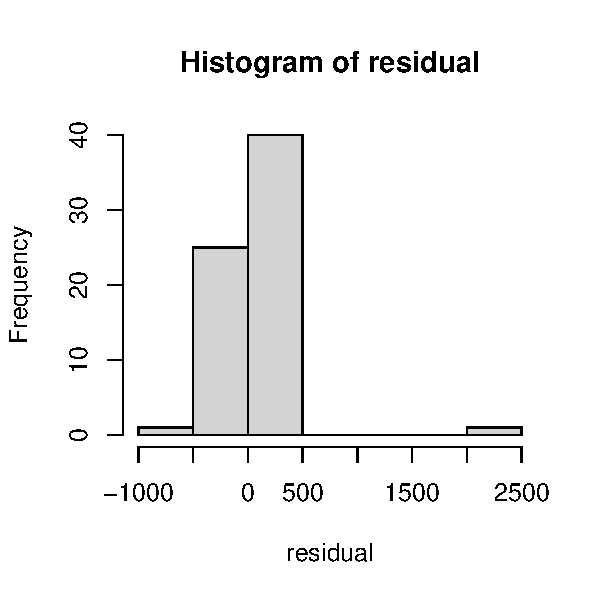
\includegraphics[width=\maxwidth]{figure/unnamed-chunk-22-1} 

}


\end{knitrout}

It looks like there is one county with a large residual.
\begin{knitrout}
\definecolor{shadecolor}{rgb}{0.969, 0.969, 0.969}\color{fgcolor}\begin{kframe}
\begin{alltt}
\hlkwd{plot}\hlstd{(florida}\hlopt{$}\hlstd{Reg.Reform, florida}\hlopt{$}\hlstd{Buch.Votes,}
     \hlkwc{main} \hlstd{=}\hlstr{"200 Presidential Election Florida Votes"}\hlstd{,}
     \hlkwc{xlab} \hlstd{=} \hlstr{"Reform Party Reg. Voters"}\hlstd{,} \hlkwc{ylab} \hlstd{=} \hlstr{"Reform Party Votes"}\hlstd{)}
\hlkwd{abline}\hlstd{(}\hlkwc{a} \hlstd{= b1.hat,} \hlkwc{b} \hlstd{= b1.hat,}
       \hlkwc{col} \hlstd{=} \hlstr{"blue"}\hlstd{,} \hlkwc{lwd} \hlstd{=} \hlnum{2}\hlstd{)}

\hlkwd{segments}\hlstd{(}\hlkwc{x0} \hlstd{= florida}\hlopt{$}\hlstd{Reg.Reform,} \hlkwc{y0} \hlstd{= florida}\hlopt{$}\hlstd{Buch.Votes,}
         \hlkwc{x1} \hlstd{= florida}\hlopt{$}\hlstd{Reg.Reform,} \hlkwc{y1} \hlstd{= y.hat,} \hlkwc{col} \hlstd{=} \hlstr{"red"}\hlstd{,} \hlkwc{lty} \hlstd{=} \hlnum{2}\hlstd{)}
\end{alltt}
\end{kframe}

{\centering 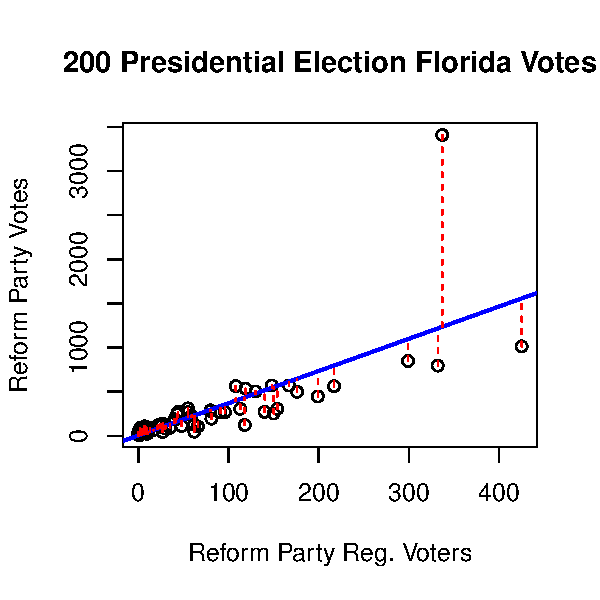
\includegraphics[width=\maxwidth]{figure/unnamed-chunk-23-1} 

}


\begin{kframe}\begin{alltt}
\hlcom{# get the name of the county with a large residual}
\hlcom{# which.max/which.min returns the index of the max/min value in the vector}
\hlstd{florida}\hlopt{$}\hlstd{County[}\hlkwd{which.max}\hlstd{(}\hlkwd{abs}\hlstd{(residual))]}
\end{alltt}
\begin{verbatim}
## [1] "Palm"
\end{verbatim}
\end{kframe}
\end{knitrout}



\subsubsection*{Questions}
\begin{itemize}
\item Does Palm County appear to be an outlier in the joint distribution? 
\item Based on the number of registered voters belonging to the reform party in Palm County, what is the fitted the number of actual votes for Pat Buchanan to be?
\item What is the residual for Palm County? (hint: Palm County is the 50th row in our data.frame)
\end{itemize}


There's a very useful function in \texttt{R} called \texttt{summary}, which we've already seen from last lab. We can also use ``summary" to our \texttt{regression.model} which gives us more information than just the raw output. Notice that it gives estimates for the coefficients, as well as standard errors for the coefficients. Recall in class that we said the estimated $\hat a$ and $\hat b$ are just estimates (statistics) of a parameter. The standard errors are rough estimates of how much our estimates might change if we took another sample. Recall the excercise above where we took samples of 10 Buffalo Bills players, and each sample gave a different result. The standard error is an estimate of the standard deviation of the histograms we were able to plot.

\begin{knitrout}
\definecolor{shadecolor}{rgb}{0.969, 0.969, 0.969}\color{fgcolor}\begin{kframe}
\begin{alltt}
\hlkwd{summary}\hlstd{(florida.regression)}
\end{alltt}
\begin{verbatim}
## 
## Call:
## lm(formula = Buch.Votes ~ Reg.Reform, data = florida)
## 
## Residuals:
##     Min      1Q  Median      3Q     Max 
## -538.89  -66.07   15.64   39.77 2176.50 
## 
## Coefficients:
##             Estimate Std. Error t value Pr(>|t|)    
## (Intercept)  -0.2464    46.7415  -0.005    0.996    
## Reg.Reform    3.6521     0.4099   8.909 7.16e-13 ***
## ---
## Signif. codes:  0 '***' 0.001 '**' 0.01 '*' 0.05 '.' 0.1 ' ' 1
## 
## Residual standard error: 302.7 on 65 degrees of freedom
## Multiple R-squared:  0.5498,	Adjusted R-squared:  0.5429 
## F-statistic: 79.37 on 1 and 65 DF,  p-value: 7.159e-13
\end{verbatim}
\end{kframe}
\end{knitrout}

Let's view the effect of Palm county on the regression and fit another model to the new data. 


\begin{knitrout}
\definecolor{shadecolor}{rgb}{0.969, 0.969, 0.969}\color{fgcolor}\begin{kframe}
\begin{alltt}
\hlstd{no.palm.county} \hlkwb{<-} \hlstd{florida[}\hlopt{-}\hlnum{50}\hlstd{, ]}
\hlstd{florida.regression.no.palm} \hlkwb{<-} \hlkwd{lm}\hlstd{(Buch.Votes}\hlopt{~}\hlstd{Reg.Reform,} \hlkwc{data} \hlstd{= no.palm.county)}
\hlkwd{summary}\hlstd{(florida.regression.no.palm)}
\end{alltt}
\begin{verbatim}
## 
## Call:
## lm(formula = Buch.Votes ~ Reg.Reform, data = no.palm.county)
## 
## Residuals:
##     Min      1Q  Median      3Q     Max 
## -210.38  -38.58  -11.76   34.49  254.65 
## 
## Coefficients:
##             Estimate Std. Error t value Pr(>|t|)    
## (Intercept)  48.8089    12.4691   3.914 0.000222 ***
## Reg.Reform    2.4031     0.1164  20.648  < 2e-16 ***
## ---
## Signif. codes:  0 '***' 0.001 '**' 0.01 '*' 0.05 '.' 0.1 ' ' 1
## 
## Residual standard error: 80.03 on 64 degrees of freedom
## Multiple R-squared:  0.8695,	Adjusted R-squared:  0.8674 
## F-statistic: 426.3 on 1 and 64 DF,  p-value: < 2.2e-16
\end{verbatim}
\end{kframe}
\end{knitrout}

Let's view the predicted vs observed values without Palm county. Here we can see that the line seems to fit the data much better than before.
\begin{knitrout}
\definecolor{shadecolor}{rgb}{0.969, 0.969, 0.969}\color{fgcolor}\begin{kframe}
\begin{alltt}
\hlkwd{plot}\hlstd{(}\hlkwc{x} \hlstd{= no.palm.county}\hlopt{$}\hlstd{Reg.Reform,}
     \hlkwc{y} \hlstd{= no.palm.county}\hlopt{$}\hlstd{Buch.Votes,}
     \hlkwc{main} \hlstd{=} \hlstr{"Registered Voters vs Actual Votes (No Palm County)"}\hlstd{,}
     \hlkwc{xlab} \hlstd{=} \hlstr{"Registered Reform Voters"}\hlstd{,} \hlkwc{ylab} \hlstd{=} \hlstr{"Actual Votes"}\hlstd{)}


\hlkwd{abline}\hlstd{(}\hlkwc{a} \hlstd{= florida.regression.no.palm}\hlopt{$}\hlstd{coefficients[}\hlnum{1}\hlstd{],}
       \hlkwc{b} \hlstd{=  florida.regression.no.palm}\hlopt{$}\hlstd{coefficients[}\hlnum{2}\hlstd{],} \hlkwc{col} \hlstd{=} \hlstr{"red"}\hlstd{)}
\end{alltt}
\end{kframe}

{\centering 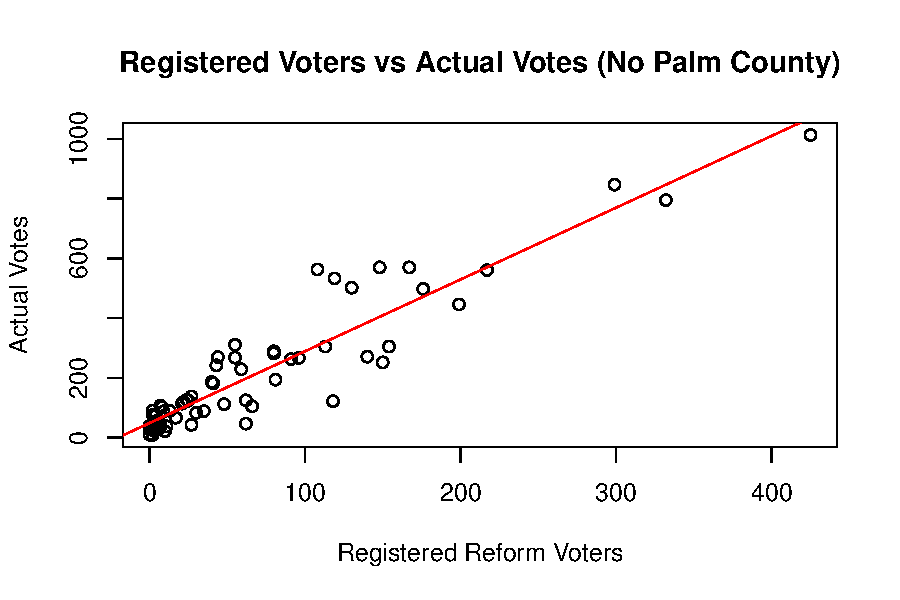
\includegraphics[width=\maxwidth]{figure/unnamed-chunk-26-1} 

}


\end{knitrout}

\subsubsection*{Questions}
\begin{itemize}
\item How would we interpret the estimated coefficients from the regression output? 
\item Using this model, what is the predicted number of votes for Buchanan in Palm County? What is the prediction error? (Note this is similar, but not a residual because we did not use Palm County to fit our model)
\item Compare the estimated values for this model with the estimated values of the previous model
\item So which model is ``correct"? The answer depends on how we define ``correct," but if you had to predict the number of votes in each Florida county for the reform party candidate in this upcoming 2024 election, which model would you use? Why?
\end{itemize}

\end{document}
